\subsection{Significado de equilibrio}

El equilibrio es un conjunto de variables seleccionadas e interrelacionadas, tan ajustadas entre sí que ninguna tendencia inherente a cambiar prevalece en el modelo que constituyen. La palabra \textit{seleccionadas} subraya el hecho de que existen variables que, por elección del análisis no seran incluidas en el modelo. Es decir que el equilibrio en el estudio tiene relevancia en el contexto del conjunto de variables elegidas, si se incluyen más variables, entonces ya no se aplica el estado de equilibrio.

La palabra \textit{interrelacionadas} sugiere que, con el fin de que ocurra el equilibrio, las variables del modelo deben estar al mismo tiempo en un estado de reposo. El estado de reposo de estas variables debe ser compatible con el de las demás, sino una o varias variables cambiarian, rompiendo el estado de equilibrio.

La palabra \textit{inherente} significa que, se considera el estado de balance de las fuerzas internas del modelo, mientras que se suponen fijos los factores externos. Los parametros y las variables exógenas se tratan como constantes. 

Al ser el equiilibrio una falta de tendencia a cambiar, se denomina a los análisis que se realizan a partir de este análisis \textit{estático}.

Aunque se crea que el hecho de que el estado de equilibrio constituye un estado ideal o deseable, este tipo de conclusiones no está garantizada. La única interpretación garantizada es que un equilibrio es una situación que, de lograrse, tendería a perpetuarse, a menos de que cambien las fuerzas externas.

En esta sección se analizara el equilibrio \textit{intermedio}, el cual ocurre cuando muchas personas, cada una buscando su propio interes, chocan entre si en un sistema. Esto significa que el equilibrio intermedio no es un proceso persona, es un proceso impersonal o suprapersonal, ya que ninguna persona en particular lo decide, es la consecuencia del sistema.

\subsection{Equilibrio de mercado parcial: un modelo lineal}

En un modelo de equilibrio estático, el desafio es hallar el conjunto de variables endógenas que satisfagan la condición de equilibrio. Una vez que se hallan identificado estos valores, se satisface la condicion de equilibrio. Considere la determinacion del precio en un mercado aislado el equilibrio parcial de mercado.

\subsubsection{Construcción del modelo}

Como solo se considera un artículos, sólo se incluyen tres variables en el sistema. La \textit{cantidad demandada} del artículo \(Q_d\), la \textit{cantidad ofrecida} del artículo \(Q_s\) y su \textit{precio} \(P\).

Una vez elegidas las variables, es necesario hacer suposiciones en relación con el desempeño del mercado. Primero se especifica la condición de equilibrio. La suposición estándar es que el equilibrio ocurra en el mercado si y sólo si la \textit{demanda excedente} es cero, es decir si \(Q_d-Q_s=0\). 

Pero ahora ¿Cómo se determinan por sí mismas \(Q_d\) y \(Q_s\)? Para responder esto partimos de la suposición teórica de que a medida de que el precio aumenta, la cantidad demandada disminuye, pero la cantidad ofrecida aumenta. Es decir, la cantidad demandada \(Q_d\) es una función lineal decreciente de \(P\) y la cantidad ofrecida \(Q_s\) es una función lineal creciente de \(P\), pero con la condición de que no se ofrece ninguna cantidad a menos que el precio rebase un nivel positivo particular. Graficamente esto se vería como la figura \ref{Grafico_oferta_demanda_analisis_estático_1}.

\begin{figure}[htbp]
    \centering
    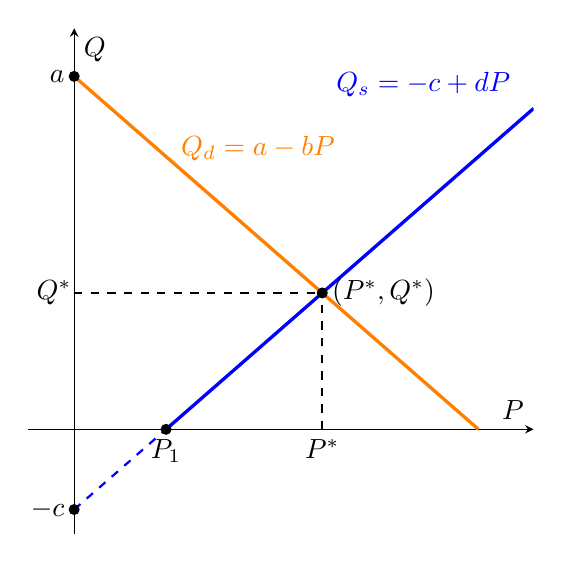
\begin{tikzpicture}
        \begin{axis}[
            axis lines = middle,
            xlabel = $P$,
            ylabel = $Q$,
            xmin=-0.5, xmax=5,
            ymin=-1.3, ymax=5,
            grid = major,
            major grid style= {dotted},
            width=8cm, height=8cm,
            ytick = \empty, xtick = \empty,
        ]
        
        % 1. TRAMO PUNTEADO: De P=0 hasta P=1 (desde -c hasta P1)
        \addplot [
            domain=0:1, 
            samples=2, 
            color=blue, 
            thick, 
            dashed
        ] {x-1};

        % 2. TRAMO SÓLIDO: De P=1 en adelante
        \addplot [
            domain=1:5, 
            samples=2, 
            color=blue, 
            very thick
        ] {x-1};

        \addplot [
            domain=4.4:0,
            samples=50,
            color=orange,
            very thick,
        ] {-1*x+4.4};

        % Etiquetas
        \node[color=blue] at (axis cs:3.8, 4.3) {$Q_s = -c+dP$};
        \node[color=orange] at (axis cs:2, 3.5) {$Q_d = a-bP$};

        % Puntos
        \fill (0,-1) circle (2 pt) node[left] {$-c$};
        \fill (0,4.4) circle (2 pt) node[left] {$a$};
        \fill (1,0) circle (2 pt) node[below] {$P_1$};

        % --- PUNTO DE EQUILIBRIO Y PROYECCIONES ---
        % Definimos las coordenadas del equilibrio (P=2.7, Q=1.7)
        \coordinate (E) at (axis cs:2.7, 1.7);
            
        % Línea punteada hacia el eje Y (Cantidad)
        \draw [dashed, thick] (axis cs:0, 1.7) -- (E) node[left, pos=0.03] {$Q^\ast$};
            
        % Línea punteada hacia el eje X (Precio)
        \draw [dashed, thick] (axis cs:2.7, 0) -- (E) node[below, pos=0] {$P^*$};
            
        % El punto físico del equilibrio
        \fill[black] (E) circle (2pt) node[right] {$(P^\ast, Q^\ast)$};

        \end{axis}
    \end{tikzpicture}
    \caption{Determinación de precio y cantidad en un mercado.}
    \label{Grafico_oferta_demanda_analisis_estático_1}
\end{figure}


De esta forma el modelo contiene una condición de equilibrio más dos ecuaciones de comportamiento que gobiernan la demanda y proporcionan los apsectos del mercado. Traducido matematicamente, el modelo se puede escribir como 

\begin{equation}
\label{Equilibrio_modelo_lineal_ecuacion_1.1}
\begin{aligned}
& Q_d = Q_s \\
& Q_d = a - bP \quad (a,b > 0) \\
& Q_s = -c + dP \quad (c,d > 0)
\end{aligned}
\end{equation}

En las dos funciones lineales aparecen parámetros, estos parámetros \((a,b,c,d)\) son positivos. Cuando se grafica la función de demanda (figura holamundo), su intersección vertical está en \(a\) y su pendiente es \(-b\), que es negativa. La función de oferta tiene una pendiente positiva \((dP)\) y su intersección vertical en \(-c\) esto para forzar a la curva de la oferta a tener una intersección horizontal positiva en \(P_1\), lo cual significa que ningun productor va a estar dispuesto a realizar y comercializar el producto si su precio se encuentra por debajo del \textit{precio minimo} \((P_1)\)

A diferencia de la práctica usual, el precio no se grafico sobre el eje vertical. Esto se debe a que por convención matemática se debe colocar la variable \textit{dependiente}(en este caso \(Q\)) en el eje vertical. En otro contexto en el cual se considera la curva de la demanda como descripcion de la curva de ingreso promedio, se invertián los ejes y se graficará a \(P\) sobre el eje vertical.

Ya con el modelo construido, el siguiente paso es resolverlo, es decir, obtener los valores de las tres variables endógenas \(Q_d, Q_s\) y \(P\). Los valores solución son los que satisfacien de forma simultánea las tres ecuaciones de \ref{Equilibrio_modelo_lineal_ecuacion_1.1}, es decir, son los valores que, cuando se sustituyen en las tres ecuaciones, las convierten en un conjunto de expresiones verdaderas. En contexto de un modelo de equilibrio, esos valores se pueden llamar \textit{valores de equilibrio} de las variables mencionadas.

En general, para denotar los \textit{valores de solución} de las variables endógenas, no se utilizan simbolos especiales. Por lo tanto simbolos como \(Q_d\) se usa para representar la variable o su valor de solución, lo mismo con \(Q_s\) y \(P\). Esta práctica puede dar lugar a confusiones, por lo tanto para evitar tal fuente de confusión, se va a denotar el \textit{valor de solución} de una variable endógena con un \textit{asterisco}. Así, los valores de solución de \(Q_d, Q_s\) y \(P\) se denotan mediante \(Q_d^\ast, Q_s^\ast\) y \(P^\ast\). 

Como el valor de solución de \(Q_d^\ast = Q_s^\ast\), podemos remplazar la expresion con un solo símbolo \(Q^\ast\). Por lo tanto, una solución de equilibrio del modelo se puede denotar mediante un par ordenado \((P^\ast,Q^\ast)\). En caso de que la solución no sea única, varios pares ordenados pueden satisfacer el sistema de ecuaciones simultáteas, entonces habrá un conjunto solución con más de un elemento. Aunque la situación de equilibrio múltiple no surge en un modelo lineal.


\subsubsection{Solución mediante eliminación de variables}

Una forma de encontrar una solución para un sistema de ecuciones es mediante la eliminación sucesiva de variables y ecuaciones por sustitución. Este modelo se constituye de tres ecuaciones (\ref{Equilibrio_modelo_lineal_ecuacion_1.1}), pero como \(Q_d = Q_s\), podemos reescribir el modelo utilizando \(Q=(Q_d=Q_s)\), lo cual nos quedaria como
\begin{equation}
    \label{Equilibrio_modelo_lineal_ecuacion_1.2}
    \begin{aligned}
    Q &= a-bP \\
    Q &= -c+dP
    \end{aligned}
\end{equation} 

Si sustituimos la primera ecuación en la segunda, el modelo se reduce a solo una ecuación con una variable
\[
a-bP = -c+dP 
\]
Luego de restar \(a=dP\) de ambos lados de la ecuación y multiplicar por \(-1\) nos quedaria\footnote{Esto es el llamado despeje, realmente no despejamos ninguna ecuación, lo que hacemos es restar y sumar variables de ambos lados, hasta llegar a una igualdad que nos sea util. La ecuación nace del principio de igualdad, si de un lado restamos una variable, del otro también, para mantener esa igualdad.} 
\begin{equation}
    \label{Equilibrio_modelo_lineal_ecuacion_1.3}
    \begin{aligned}
    (b+d)P = a+c
    \end{aligned}
\end{equation}

Este resultado se podria obtener directamente de \ref{Equilibrio_modelo_lineal_ecuacion_1.1} si sustituimos las ecuaciones segunda y tercera en la primera.

Como \(b+d \neq 0\), es valido dividir de ambos lados de \ref{Equilibrio_modelo_lineal_ecuacion_1.3} entre \(b+d\). El resultado es el valor de solución \(P\), es decir 
\begin{equation}
    \label{Equilibrio_modelo_lineal_ecuacion_1.4}
    \begin{aligned}
    P^\ast=\frac{a+c}{b+d}
    \end{aligned}
\end{equation} 

\(P^\ast\) se expresa en términos de los parámetros que representan los datos del modelo. \(P^\ast\) es un valor definido y positivo (como debe ser el precio), debido a que todos los parametros son positivos por especificación del modelo.

Para encontrar el valor de solución de la cantidad de equilibrio, es decir \(Q^\ast\) que corresponde al valor \(P^\ast\), se sustituye la ecuación \ref{Equilibrio_modelo_lineal_ecuacion_1.4} en cualquier ecuación de \ref{Equilibrio_modelo_lineal_ecuacion_1.2}, y luego se soluciona la ecuación resultante. Hagamos el procedimiento, partamos de que 
\[
    Q^\ast=a-bP
\]
Como \(P = (a+c)/(b+d)\), se puede replazar en la expresión anterior, resultando
\[
Q^\ast=a-b(\frac{a+c}{b+d})
\]
Ahora multiplicamos a \(a\) por \(1\)
\[
Q^\ast=a(1)-b\frac{a+c}{b+d}
\]
Pero como \(1\) es lo mismo que decir \((b+d)/(b+d)\), es decir \(1=(b+d)/(b+d)\) ya que si realizamos la fracción su resultado va a ser \(1\). Nos queda que 
\[
Q^\ast=a\frac{b+d}{b+d}-b\frac{a+c}{b+d}
\]
Que es lo mismo que decir que 
\[
Q^\ast= \frac{a(b+d)}{b+d}-\frac{b(a+c)}{b+d}
\]
Recordando que matemáticamente \(1/2 + 3/2 = 4/2\), podemos hacer lo mismo en nuestra ecuación, dandonos 
\[
Q^\ast= \frac{a(b+d)-b(a+c)}{b+d}
\]
Realizando la distributiba, nos queda 
\[
Q^\ast= \frac{ab+ad-ba-bc}{b+d}
\]
Y como \(ab = ba\) estos se anulan, quedandonos 
\[
Q^\ast= \frac{ad-bc}{b+d}
\]
Que al igual que \(P^\ast\) es una expresión sólo en términos de parámetros. Como el denominador \(b+d\) es positivo, \(Q^\ast\) requiere que el número de \(ad-bc\) sea positivo también. Es decir que para que tenga significado económico, el modelo tiene la restricción de que \(ad>bc\).

El significado de esta restricción se puede ver en la figura \ref{Grafico_oferta_demanda_analisis_estático_1}. Para obtener la intersección económica de \(P^\ast\) y \(Q^\ast\), se requiere que \(Q^\ast\) sea mayor que \(0\), lo cual significa que debe estar localizado por encima del eje horizontal de la figura \ref{Grafico_oferta_demanda_analisis_estático_1}, esta restricción que encontramos en la teória y en el gráfico es la que mencionamos anteriormente \(ad>bc\).

La intersección de las curvas de oferta y demanda no es diferente al concepto de intersección visto en conjuntos. Por lo tanto esto expresado en forma de conjuntos (que es lo que son tanto \(Q_s\) y \(Q_d\)), nos queda que

\begin{equation}
    \begin{aligned}
    D (\text{demanda}) &= \{(P,Q) | Q = a - bP\} \\
    S (\text{oferta}) &= \{(P,Q) | Q = -c + dP\} \\
    \end{aligned}
\end{equation} 

Por lo tanto la intersección de la oferta y la demanda se expresaria como
\[
D \cap S = \{(P^\ast,Q^\ast)\}
\]
El conjunto intersección contiene un sólo elemento, el par ordenado \(P^\ast, Q^\ast\), lo que quiere decir que el equilibrio del mercado es único.

\begin{ejercicio}
    \begin{enumerate}
        \item Dado el modelo de mercado
        \begin{equation}
            \begin{aligned}
            Q_d &= Q_s \\
            Q_d &= 21-3P \\
            Q_s &= -4+8P
            \end{aligned}
        \end{equation} 
        Obtenga \(P^\ast\) y \(Q^\ast\) por \((a)\) eliminacion de variables y \((b)\) por medio de las formulas \(P^\ast=(a+c)/(b+d)\) y \(Q^\ast= (ad-bc)/(b+d)\). (Use fracciones en vez de decimales).
        \item Sean las funciones de la oferta y la demanda como siguiente
        \begin{equation}
            \begin{aligned}
            Q_d &= 51-3P \qquad \qquad Q_d &= 30-2P \\
            Q_s &= 6P-10 \qquad \qquad Q_s &= -6+5P 
            \end{aligned}
        \end{equation} 
        Determine \(P^\ast\) y \(Q^\ast\) mediante la eliminación de variables.
        \item Si \(b+d = 0\) en el modelo de mercado lineal, ¿Se puede encontrar una solución de equilibrio al usar \(P^\ast=(a+c)/(b+d)\) y \(Q^\ast= (ad-bc)/(b+d)\)?¿Por qué?
        \item Si \(b+d = 0\) en el modelo de mercado lineal, ¿Qué se puede concluir en relación con las posiciones de las curvas de demanda y equilibrio en la figura \ref{Grafico_oferta_demanda_analisis_estático_1}?¿Qué concluye entonces con respecto a la solución del equilibrio?
    \end{enumerate}
    \emph{Respuestas}
    \begin{enumerate}
        \item Antes de dar los resultados, me gustaria aclarar la analogía. Qué nos dice \(Q_d=21-3P\), nos dice que si el precio fuera \(0\), \(21\) personas estarian dispuestas comprar el producto, y el \(-3\) nos dice que tan sensible es la gente al precio, por cada \(\mathdollar{1}\) perderiamos \(3\) clientes.
        
        En el caso de la oferta \((Q_s)\), el \(-4\) nos indica que para empezar la producción necesitamos un precio que supere ese nivel, y en el caso de \(8\) indica que por cada \(\mathdollar{1}\) adicional, estamos dispuestos a ofrecer 8 productos más.

        Solución:
        $$
        \begin{aligned}
        P^* &= 25/11 \\
        Q^* &= 156/11
        \end{aligned}
        $$
        \item Solución:
        $$
        \begin{aligned}
        P_1* &= 61/9 \qquad \quad P_2^* &&= 36/7\\
        Q_1^* &= 92/3 \qquad \quad Q_2^* &&= 138/7
        \end{aligned}
        $$
        \item Matemáticamente no, no se puede encontrar una solución de equilibrio mediante esas fórmulas, ya que la división por cero no está definida.
        \item Gráficamente van a ser lineas paralelas que nunca se van a cruzar. Económicamente significa que no existe ningún precio en el que los deseos de los compradores coincidan con los de los vendedores.
    \end{enumerate}
\end{ejercicio}